\section{Background}

\cloakingTypes



Over past several decades, the anti-phishing ecosystem has proposed and leveraged a number of techniques to detect and migitate phishing attacks~\cite{oest2018inside}.
Techniques such as URL~\cite{bin2010dns, blum2010lexical, huang2012svm, khonji2011novel} and web page content analysis~\cite{wu2006web, zhang2007cantina, zhang2011textual, bilge2011exposure, canali2013role} have raised the defensive level of the ecosystem and productized implementations such as URL blacklists, malicious infrastructure analysis, and e-mail spam filter.

Commodity URL blacklists such as Google Safe Browsing~\cite{whittaker2010large} and Microsoft SmartScreen~\cite{smartscreen} reinforces the backend of the anti-phishing ecosystem, which warn users with prominent sign indicating that the websites ahead are suspicious when phishing URL is detected and blacklisted.
Evasion techniques, also known as cloaking techniques, are widely leveraged in phishing attacks to delay or disable detection by anti-phishing systems~\cite{liang2016cracking, oest2019phishfarm, oest20phishtime}.

\subsection{Server-side Cloaking in Phishing}


Attackers often implement \emph{cloaking techniques} to evade detection by the anti-phishing ecosystem.
Typically, phishing websites with evasion display benign web page content if they suspect the visit originates from a security infrastructure~\cite{wu2005cloaking}.
There are two categories of cloaking techniques, namely server-side and client-side (\autoref{tab:cloakingtypes} shows categories of each type).
Client-side evasion techniques distinguish visitors to display different web page content by executing JavaScript snippets in user's browser~\cite{zhang2021crawlphish}.
Server-side cloaking techniques, on the other hand, identify visits from anti-phishing systems through information in HTTP requests~\cite{oest2018inside, invernizzi2016cloak}.
Typically, server-side cloaking is also known as fingerprinting cloaking, including network, browser, and context~\cite{invernizzi2016cloak}.
\autoref{fig:fp_cloaking} shows how fingerprinting cloaking techniques are used in phishing websites.
Cloaking code embedded in the phishing server fingerprints the profile in the HTTP request and responds different web page content based on the identification of visitors (as either potential victims or anti-phishing crawlers).

Researchers detect and categorize client-side cloaking techniques in phishing by force-executing the payload JavaScript snippets~\cite{zhang2021crawlphish}.
To bypass server-side cloaking techniques in phishing attacks, the anti-phishing systems camouflage themselves as if they are regular visitors.
Only when anti-phishing systems retrieve phishing content, can they classify phishing websites~\cite{xiang2011cantina+,whittaker2010large,smartscreen}.

However, as the development of phishing kits, the size of blocklist in the phishing kit increases.
As shown in~\autoref{fig:servercloaking}, any match of the IP addresses or hostnames in the blocklist will result in an error web page, such as 404 Page Not Found.
Hence, anti-phishing systems can trigger fingerprinting cloaking techniques in the phishing server easily.
As a result, they cannot properly retrieve phishing web page content, which leads to a mis-classification.
Moreover, according to the analysis from Oest et al.~\cite{oest2020sunrise}, it takes anti-phishing crawlers an average of six hours to mark a phishing website as malicious.
The duration is even longer till the last victim visit (18 hours).
Such long reaction time has left phishers a golden hour to hurt Internet users.

We can consider the problem from a different angle: phishers try their best to evade visits from anti-phishing ecosystem, so how about Internet users camouflage themselves as crawlers when visiting phishing websites?
In this way, users can only see an error web page and never submit credentials to phishers.
It also shrinks the reaction time to blacklist them.


% \subsection{Mitigations Against Advanced Phishing}

% \subsection{Limitations of Mitigations}

\begin{figure}
\centering
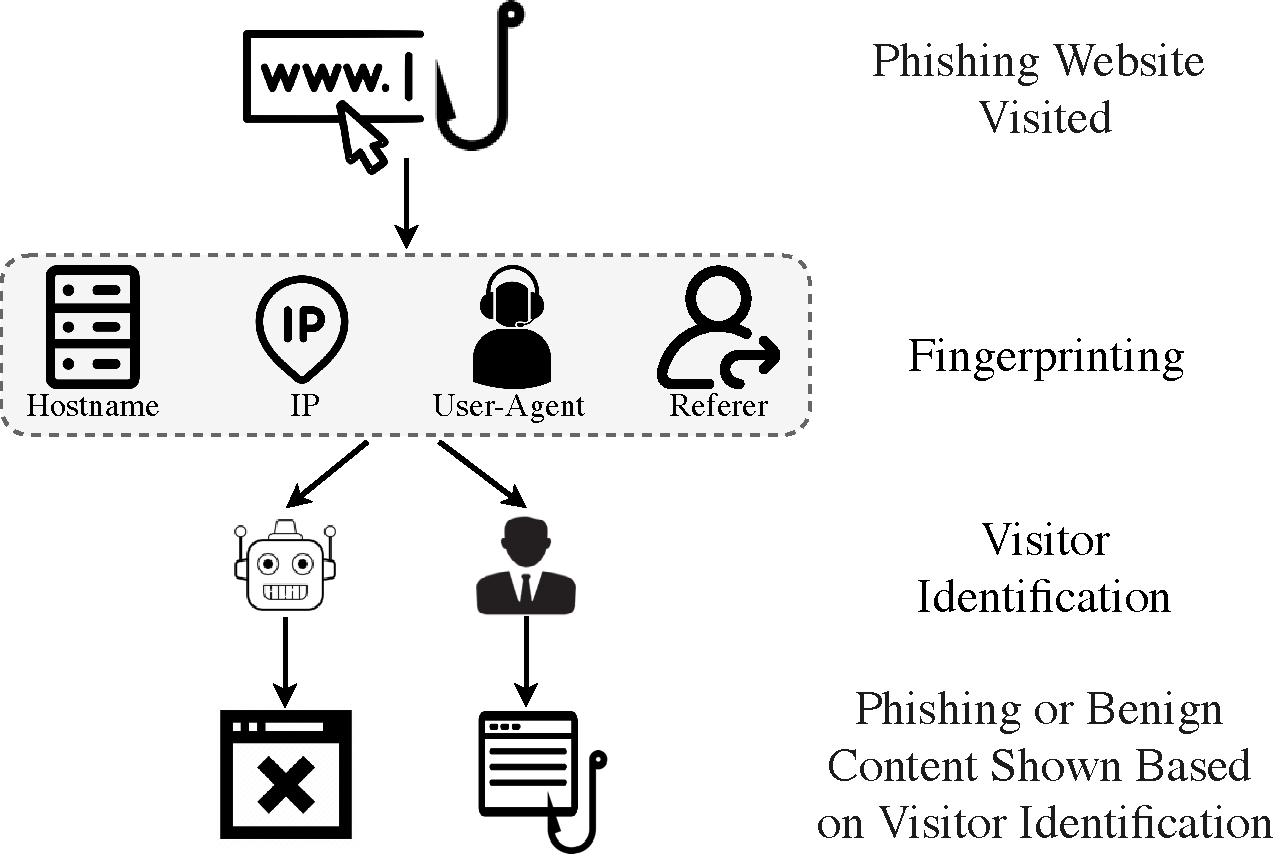
\includegraphics[width=.9\linewidth]{figs/fp_cloaking.pdf}
\caption{Typical operation of fingerprinting cloaking in phishing websites.}
\label{fig:fp_cloaking}
% \vspace{-15pt}
\end{figure}